\documentclass[12pt]{article}

\usepackage[utf8]{inputenx}
\usepackage[spanish]{babel}
\usepackage[top=1.5cm, bottom=1.5cm, left=1.5cm, right=1.5cm]{geometry}
\usepackage{graphicx}
\usepackage[T1]{fontenc}
\usepackage{lmodern}
\usepackage{LobsterTwo}
\usepackage{tikz}
\usepackage{lipsum}
\usepackage{multicol}

\usepackage{fancyhdr}
 


\renewcommand{\familydefault}{\sfdefault}


%.............. Definicion de \maketitle
\newcommand{\subject}[1]{#1}
\makeatletter
\renewcommand{\maketitle}{

{\centering \begin{minipage}[b]{\hsize}	

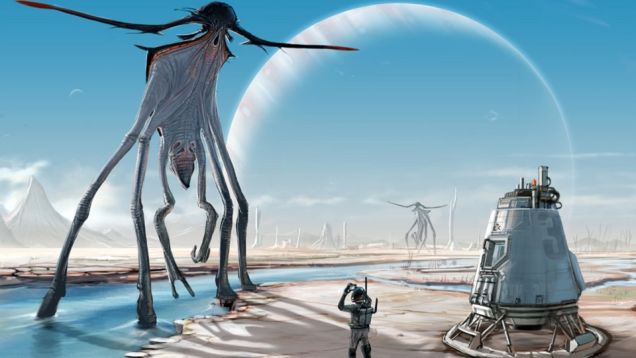
\includegraphics[width=\hsize]{portada}

Foto: \emph{Xenobiology} by Abiogenesis on DeviantArt.

\end{minipage} 
}
\vspace{0.5cm}

\bgroup
%algo sobre Alineacion del texto

{\LobsterTwo \huge \raggedright \@title}
\vspace{0.4cm}

{\Large \raggedright  \@author} \\
{\raggedright \large Laboratorio de Divulgación de la Ciencia}

\egroup

\begin{center}
 \tikz \draw[thick,double](0,0)--(\hsize,0 );	
\end{center}




}
\makeatother

%...............................................


\title{ De la paradoja de Fermi \\ 
y el nuevo optimismo por la vida extraterrestre}
\author{M. F. Pérez-Ramírez}
\date{}


\pagestyle{empty}
\fancyhf{}


\begin{document}
\maketitle

\begin{minipage}[c]{10.0cm}
	Prueba de minipage:
	Desde siempre, la \emph{soledad} me ha parecido un concepto interesante. Incluso para los que preferimos la compañía de pocos amigos, o los que nos sentimos más cómodos en ambientes donde no nos vemos forzados a convivir
\end{minipage}

\begin{multicols}{2}



Desde siempre, la \emph{soledad} me ha parecido un concepto interesante. Para los que preferimos la compañía de pocos amigos, o los que nos sentimos más cómodos en ambientes donde ser \emph{introvertido} no está mal visto, \emph{estar solo} adquiere un significado más profundo, a veces oscuro. \\

Estar solo no se trata de 


\end{multicols}






\end{document}